
\section{Summary of results}
Correlations between model fitness and model parameters:

However, the deeper analysis showed that even though correlation existed between some of the population wide parameter averages\footnote{Reminder: population wide refers to calculating the average of the fitness or parameter over all simulations that ever existed in the genetic algorithm} and some of the model fitnesses, there were also several exceptions.

Faster market makers can have negative effects on the market.
-Longer to become stable (when few chartists)
-increased overshoot, although very slight (when few chartists) When many chartists, fast market makers prevent a large overshoot.
-increased flickering of prices (stronger with few chartists). However, when many chartists, market makers must be fast to keep market from overflickering.
-longer time to reach the new fundamental (stronger with many chartists) (clear tendency)
\begin{comment}
\begin{figure}
\centering
\subcaptionbox{}[0.49\linewidth]{\includegraphics[width=0.5\textwidth]{}}
\subcaptionbox{Experiment \dnine}[0.49\linewidth]{\includegraphics[width=0.5\textwidth]{103_scatter_manual_outlier/d9/k.png}}
\subcaptionbox{Experiment \dten}[0.49\linewidth]{\includegraphics[width=0.5\textwidth]{103_scatter_manual_outlier/d10/h.png}}
\subcaptionbox{Experiment \dten}[0.49\linewidth]{\includegraphics[width=0.5\textwidth]{103_scatter_manual_outlier/d10/k.png}}
\subcaptionbox{Experiment \deleven}[0.49\linewidth]{\includegraphics[width=0.5\textwidth]{103_scatter_manual_outlier/d11/h.png}}
\subcaptionbox{Experiment \deleven}[0.49\linewidth]{\includegraphics[width=0.5\textwidth]{103_scatter_manual_outlier/d11/k.png}}
\caption{Scatter plot of $\log \stdev$ against \timetoreachnewfundamental with coloring showing $\roundstable$ and \overshoot}
\label{figure:d9_scatter_fitness_inliers_b}
\end{figure}
\end{comment}




The results in the previous chapter show that the latency of the HFT agents have a definite impact on the way that the market behaves. However, the results show that the model is no

Some markets may benefit from having fast agents, while other markets may not. Whether or not a market benefits from having fast traders, and the way in which it does, was shown to depend on several factors. In particular the ratio between the number of the two types of fast traders, and their relative speeds 


However, the number of orders submitted by slow traders is also of significant importance, as they determine the force that drives that market towards the true fundamental price.

Ideally


\section{Predictability of market behavior}
In the previous chapter it was also shown that markets with the same parameter could show significantly varying behavior. The model contains a large number of random factors. First of all, most of the model parameters are merely parameters in probability distributions that are sampled within the model. For instance, \ssmmlatencymu{} and \ssmmlatencys{} do not determine how fast each agent will be, but merely determine the distribution of the latency parameters of the population of market makers in the model. Evaluated with the same parameters, some markets may have a few market makers with almost no latency, while others may contain only slow market makers. 

In the case of market makers, it was observed that the population wide average fitness values for markets containing calculated over the entire pup

One example of this 

This unpredictable behavior causes the analysis to be more complex. Yet, in spite of this fact, correlations were found between most of the parameters and the model fitness.












\section{Summary of results}
\begin{itemize}
\item Markets with many market makers tended to be slow and stable, while market with few market makers tended to be fast and unstable. Chartists had the opposite effect, such that market with many chartists were fast and unstable, and markets with few chartists were slow and stable.
\item Markets with many chartists compared to market makers 

\item In markets with many chartists, fast market makers make the market respond slowly to the shock. For instance, in the case of the market having between 100 to 1250 chartists, the 

reduces the overshoot and the price flickering, but also makes the market take more rounds to reach the new fundamental. HoweverMarkets which had many chartists but only slow market makers had an even larger overshoot and highly flickering prices, but managed to reach the new fundamental faster. Hence, fast market makers did provide some benefits in this case.



\end{itemize}


\subsubsection*{Impact of market maker latency in markets with many chartists}
In general, the difference between the fitness values of markets with fast market makers and slow market makers is largest when the market also has a large number of chartists. 


This is especially true for the responsiveness of the markets with \ssmmlatencymu close to zero on average take around 18000 rounds to reach the new fundamental, while markets with \ssmmlatencymu only take around 12000 rounds (yellow line on figure \ref{fig:faster_mm_makes_worse_markets_SC_a}). In comparison, the responsiveness for market with less than 25 chartists only decreased around 9.5\% (red line).

\subsubsection*{Impact of market maker latency in markets with few chartists}
Surprisingly

The ratio between the number of chartists and market makers have a large impact on the behavior of the market. In addition, the latency of each agent type influence the market in different ways. 

Curiously enough, the market has a smaller overshoot for $0 < r < 0.6$ when the chartists are slow, as the red line on figure \ref{fig:latency_vs_fitness_with_lines_for_agent_ratio_overshoot_mmlatency} shows. As $r$ grows, slower market makers increasingly cause the market to have a larger overshoot. 

Although not shown in the figure since it would compress the plot, the overshoot grows even more for larger $r$. 

Hence, in market where there are relatively few chartists, even the slow market makers are able to keep the market from overshooting, no matter how fast the chartists are. This is even true when there are roughly as many chartists as there are market makers in the model.

When the number of chartists is kept fixed, 






\subsection{Agent latency and }

The results confirmed that crashes do not occur in markets without market makers, nor in markets without chartists. However, the results also show that crashes rarely happen, even when the market has several chartists and market makers. The two factors that turned out to be the most important for whether or not a market is in risk of crashing or not, is the ratio between the number of chartists and the number of market makers ($\rho_A$), and the ratio between the average latency of each of the two agent types $\rho_{\lambda}$.

\begin{figure}
	%issue 15
	\centering
	\subcaptionbox{}
	[0.49\linewidth]{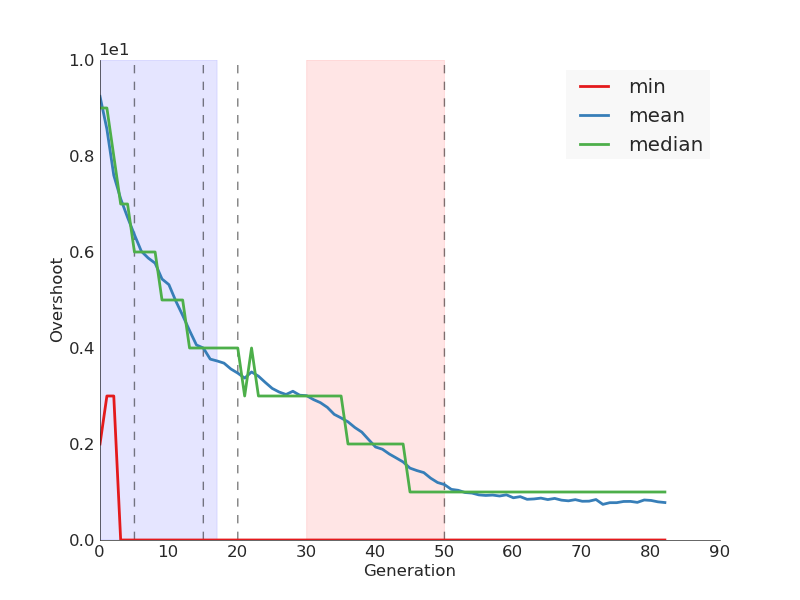
\includegraphics[width=0.5\textwidth]{manually_selected/ar_lr/overshoot.png}}
	\caption{}
	\label{}
\end{figure}


If a crash is defined 
Figure

The left figure shows how the overshoot depended on both $\rho_{\lambda}$ and $\rho_A$

The left figure shows how , while the right figure 
It turned out that the most important factor for whether or not a market would crash was 




When the market makers submit new buy orders, the have to determine a price. if they are fast they will detect the latest drops in trade prices and submit buy orders at accordingly lower prices

During this period, it may happen that the market maker will 

However, the market does no crash every time there are both chartists and market makers. On the contrary, the market proved to be fairly robust in that it did not crash very often. So waht made the market crash?


\section{Model parameters}
The model has many parameters that we did not tune.
Furthermore, the chartists submit limit orders, which means that the order book will not keep the chartist orders. 

The fundamentalists will rarely submit 



\section{Few fast mm dominating the market}
 


In the case that the best price sell side remains constant, a widening spread means that the price on the buy side is falling. Upon detecting this, the market makers will cancel their current orders and submit new buy orders at a few ticks below the previous buy price. These orders 

A widening spread means that 


% % %Hence, crashes are not cause by the market being flooded by sell orders, but rather by the sell side remaining more or less untouched, while the prices on the buy side rattles down.


with a small a spread as their strategy allows,  as long as there are other orders in the order book that 

will meet the lower prices of the orders submitted by the chartists 

However, if the market also contains market makers, crashes become more likely. 

\section{Market makers causing overevaluation}

\begin{itemize}
\item The market rarely (if ever) crashes when the x
\end{itemize}


\section{Flickering prices}

Market makers were shown to suppress price flickering. This ability of the market makers  because they only move the prices at which they have orders in the market, if 


In order for a crash to happen, 


The reason for this is that the market makers are too slow to submit enough 

\begin{figure}
	%issue 15
	\centering
	\subcaptionbox{\label{fig:latency_vs_fitness_with_lines_for_agent_ratio_overshoot_mmlatency}}
	[0.49\linewidth]{\includegraphics[width=0.5\textwidth]{latency_vs_fitness_with_lines_for_agent_ratio/d10d11/overshoot_mmlatency.png}}
	\subcaptionbox{\label{fig:latency_vs_fitness_with_lines_for_agent_ratio_overshoot_sclatency}}
	[0.49\linewidth]{\includegraphics[width=0.5\textwidth]{latency_vs_fitness_with_lines_for_agent_ratio/d10d11/overshoot_sclatency.png}}
	\caption{Average overshoot as a function of agent latency and ratio between the number of chartists and market makers}
	\label{fig:faster_mm_makes_worse_markets_SC}
\end{figure}

Benefits of markets with fast agents


Benifits of markets with many 

Fast market makers can make the market take longer to stabilize


\section{Trader speed and market overshoot}
The trader speed did indeed have a large impact on the market overshoot
\begin{table}
\begin{tabular}{c|cc}

\toprule
&$\ssmmlatencymu < 50$&
\midrule
\overshoot & 0.23 &
\roundstable &15968 &
\stdev  &  0.74 &
\timetoreachnewfundamental &  19282 &
\bottomrule
\end{tabular}
\caption{title}
\end{table}
many fast chartists
many slow chartists
few fast chartists 
few slow chartists
\section{Trader speed and price stability}


When few chartists, slower market makers were better. Faster market makers ersults in longer time to stabilize, and larger overshoot.

Trade-off between responsiveness and stability.

Refer to the section of the best individuals. 
Some simulations were fast and unstable, while others were slow and stable. Although there were models in between, no stable model managed to be as fast as another unstable model. and no fast model managed to be as stable as a stable one. 

The trade-off between these two types of behavior was shown to be 

Whether such ideal market behavior is possible within the model is doubtful. 



As was shown in figure \ref{figure:d10_fitness_correlation}, \timetoreachnewfundamental{} is negatively correlated with both \stdev{} and \overshoot{}. This is another factor that points towards the existence between responsiveness and stability. The negative correlation means that \timetoreachnewfundamental will be high when \stdev and \overshoot are low and vice versa. 
XXX: insert figure of D11 fitness correlation

\section{Consistent dynamics}

Market makers amplify the behavior

\section{Ratio of agents}
In chapter \ref{chapter:experiments_and_results} it was shown that a correlation exists between the number of high frequency traders and some of the fitness measures. 

It is possible that this evolution of the parameters is caused by the model being unable to be both fast and stable, but that there exists a trade-off between the two. Even though such a trade-off is not inherent in the model, in may happen to be inevitable when performing a parameter search, simply because the set of parameters causing the model to be both responsive and stable are so few that they are simply too difficult to find. Indeed, as is shown in section \ref{section:hall_of_fame}, no parameters caused the market to be both 


\section{Fast market makers and many chartists}
This combinations seems to drive the market to having overshoot (where's the evidence?)


\begin{figure}
\centering
\subcaptionbox{Experiment \dnine}[0.49\linewidth]{\includegraphics[width=0.5\textwidth]{par_tendencies/all/d10_overshoot_chartist_latency.png}}
\subcaptionbox{Experiment \dnine}[0.49\linewidth]{\includegraphics[width=0.5\textwidth]{par_tendencies/all/d10_overshoot_mm_latency.png}}
\subcaptionbox{Experiment \dnine}[0.49\linewidth]{\includegraphics[width=0.5\textwidth]{par_tendencies/all/d11_overshoot_chartist_latency.png}}
\subcaptionbox{Experiment \dnine}[0.49\linewidth]{\includegraphics[width=0.5\textwidth]{par_tendencies/all/d11_overshoot_mm_latency.png}}
\caption{Scatter plot of \roundstable against \timetoreachnewfundamental with coloring showing $\log \stdev$ and \overshoot}
\label{figure:scatter_fitness_inliers_a}
\end{figure}
\begin{figure}
\centering

\end{figure}

\section{Slow and fast trader order balance}
The market maker strategy is designed such that a market maker can only have a single buy order and a single sell order in place at the market at the same time. When an order submitted by market maker $i$ is filled, it takes \ssmmlatencyagent{i} rounds before the agent is notified of the result. When the market maker receives trade information, it thinks for \ssmmthinkagent{i} rounds, and then submits a new order to the market, which arrives after another \ssmmlatencyagent{i} rounds. Recall that market maker $i$ submits orders with a fixed volume, \ssmmordervolume{i}. The maximum volume that the market maker can move during $n$ rounds is therefore inversely proportional to its latency to the market:
\[\text{Maximum volume} \propto 2\ssmmlatencyagent{i} + \ssmmthinkagent{i}\]
Given that the market contains \ssmmnAgents market makers, the expected number of trades that they can 

agent latencies are IID

has to wait until it receives the new market information until it can make a decision on how to trade. Hence, the number of orders that 

\section{Better prediction accuracy in market with more and slower agents}
latency variance was independent of 

\ssmmlatencys and \sclatencys were 

When \ssmmlatencymu{} and \sclatencymu{} are small, the market is more likely to have agents with almost no latency. Such ultra fast agents have an amount of influence over the market which is disproportionate to their latency


Hence, the evidence points towards a few, very fast agents being able to ``break'' the market.
The high variance of all t

The point is that the model becomes less predictable when there is a high number of chartists. 


\section{Combination of many chartists with many market makers}
Many market makers make the market sluggish.
Make chartists make the market flicker.
But it takes many of both to create crashes.
To be clear, what is really important is the balance of total order volume by slow traders, chartists and market makers.
A market in which the collected volume HFT market makers 
Chartists are by themselves not able to create a large crash, as



\section{Strategy crowding}

\section{Between data set inconsistencies}

\section{Model assumptions}

\section{Model limitations}
The most obvious limitation imposed by the model is the small number of different agent strategies.

Another possible short-coming is the simplicity of the slow trader strategy. 